%% Conclusion figure without Python
\hypertarget{fig:conclusion-scatter-nopy}{} % anchor for links
% \begin{adjustbox}{max width=\textwidth}
    \begin{figure}[h]
        \centering
        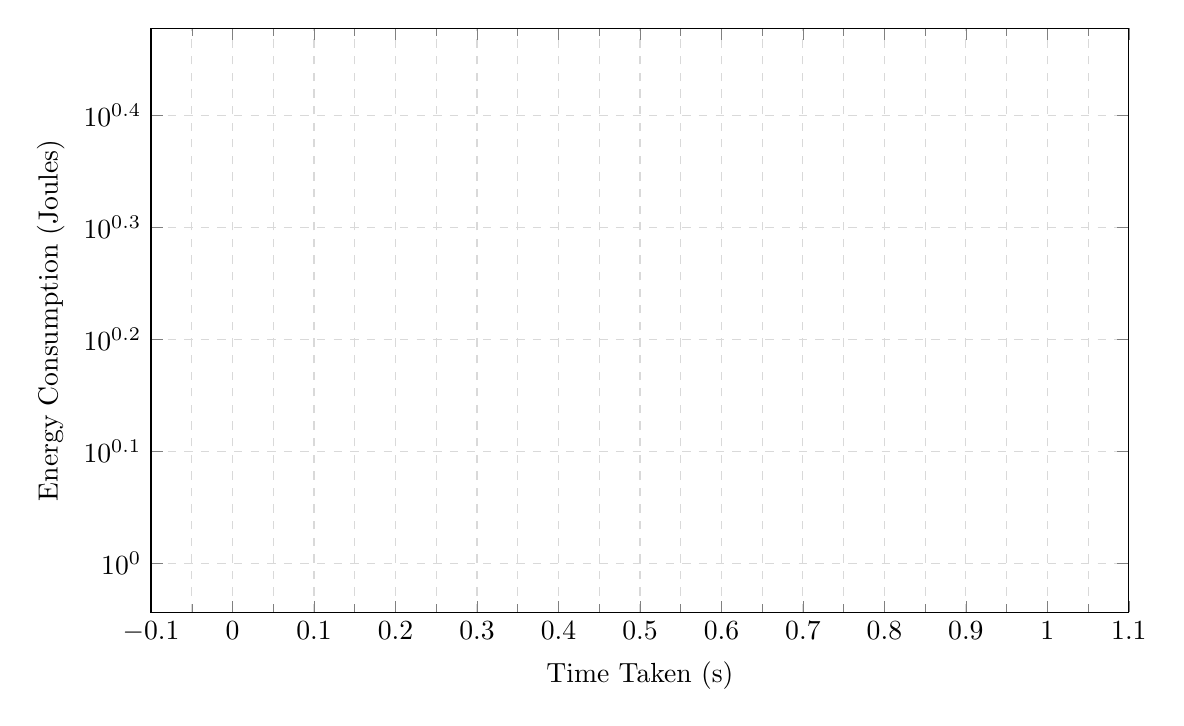
\begin{tikzpicture}
            \begin{axis}[
            width=14cm, height=9cm,
            xlabel={Time Taken (s)},
            ylabel={Energy Consumption (Joules)},
            ymode=log,
            xmin=0, xtick={0,20,40,60,80,100,120,140,160,180,200,220,240,260},
            % enlarge x limits=false,
            grid=both, minor tick num=1,
            grid style={gray!30,dashed},
            legend style={at={(0.5,1.05)},anchor=south,legend columns=-1, draw=none},
            enlargelimits=0.1,
            clip=false
            ]
            % plots (no Python)
            \PlotCXXconclusion
            \PlotGoconclusion
            \PlotPyPyconclusion
            \legend{C++, Go, PyPy}

            % clickable "button" back to the full plot
            \node[anchor=north east, fill=gray!15, draw, rounded corners,
                    inner sep=3pt] at (axis description cs:0.98,0.98)
                                {\hyperref[chap:appendix-scatter-plot]{\strut Show \emph{with} Python}};
            \end{axis}
        \end{tikzpicture}
    \caption[Scatter plot of C++, Go, and PyPy.]{The plot shows the relationship between time taken and energy consumption for each programming language. The data points represent different implementations, where the label has the form X-Y, with X being the platform and Y being the number of cores used.}
    \label{fig:conclusion-scatter-nopy}
    \end{figure}
% \end{adjustbox}